\part{Práctica 4: Pruebas del Sistema (Testing)}

\section{Introducción}

El proceso de testing constituye una fase crítica dentro del ciclo de vida del software. Según Sommerville \cite{Sommerville2015}, las pruebas no solo buscan identificar defectos, sino demostrar que el sistema cumple con los requisitos especificados y que es adecuado para su propósito. En el contexto de la metodología UWE, el testing debe verificar tanto los aspectos funcionales (derivados de los casos de uso y diagramas de actividad) como los no funcionales (rendimiento, seguridad, usabilidad).

Esta práctica aborda la \textbf{auditoría integral} del sistema QR Restaurante, aplicando técnicas de prueba sobre cinco ejes fundamentales: usabilidad e interfaz, funcionalidad, base de datos, compatibilidad y rendimiento/seguridad. El objetivo es generar evidencias objetivas que demuestren la calidad del producto desarrollado.

\section{Estrategia de Pruebas}

\subsection{Tipos de Prueba Aplicados}

\begin{figure}[hbt!]
    \centering
    \resizebox{0.7\textwidth}{!}{%
    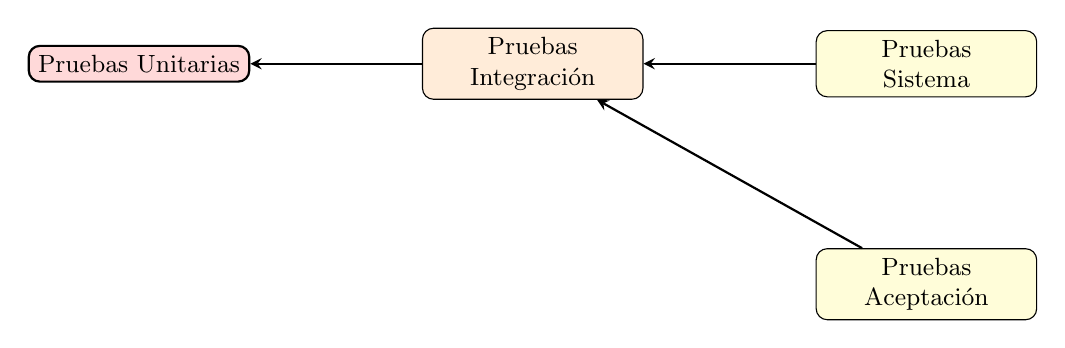
\begin{tikzpicture}[
        every node/.style={draw, rounded corners, align=center, font=\small, minimum width=2.8cm},
        nivel1/.style={fill=red!15, thick},
        nivel2/.style={fill=orange!15},
        nivel3/.style={fill=yellow!15},
        flecha/.style={->, >=stealth, thick}
    ]
    \node[nivel1] (piramide) {Pruebas Unitarias};
    \node[nivel2, right of=piramide, xshift=4cm] (integracion) {Pruebas\\Integración};
    \node[nivel3, right of=integracion, xshift=4cm] (sistema) {Pruebas\\Sistema};
    \node[nivel3, below of=sistema, yshift=-1.8cm] (aceptacion) {Pruebas\\Aceptación};

    \draw [flecha] (sistema) -- (integracion);
    \draw [flecha] (aceptacion) -- (integracion);
    \draw [flecha] (integracion) -- (piramide);
    \end{tikzpicture}
    }
    \caption{Pirámide de Testing — Estrategia aplicada.}
    \label{fig:piramide_testing}
\end{figure}

\begin{enumerate}
    \item \textbf{Pruebas Unitarias}: Verificación individual de cada componente (validación de QR, cálculo de duración, recálculo de valoración media).
    \item \textbf{Pruebas de Integración}: Validación de la interacción entre módulos (escaneo → validación → registro de visita → actualización de aforo).
    \item \textbf{Pruebas de Sistema}: Evaluación completa del sistema desplegado contra todo el catálogo de requisitos.
    \item \textbf{Pruebas de Aceptación}: Verificación final desde la perspectiva de cada perfil de usuario.
\end{enumerate}

\subsection{Técnica de Diseño de Casos de Prueba}

Se emplea la técnica de \textbf{Partición de Equivalencia} combinada con \textbf{Análisis de Valor Límite} para maximizar la cobertura con el menor número de casos:

\begin{itemize}
    \item \textbf{Partición de equivalencia:} Se agrupan entradas similares que deben producir el mismo comportamiento (por ejemplo, todos los UUIDs inválidos se tratan igual).
    \item \textbf{Valor límite:} Se prueban los casos frontera (campo vacío, máximo de caracteres, límite de capacidad, 0 acompañantes, 11 acompañantes siendo el máximo 10).
\end{itemize}

\section{Plan de Pruebas}

\subsection{Identificación de Casos de Prueba}

\begin{table}[hbt!]
    \centering
    \caption{Plan de Pruebas — Resumen de Casos}
    \label{tab:plan_pruebas}
    \begin{tabular}{|c|l|l|l|c|}
        \hline
        \textbf{ID} & \textbf{Módulo} & \textbf{Caso de Prueba} & \textbf{Tipo} & \textbf{Prioridad} \\
        \hline
        TC-01 & Registro & Registrar restaurante con datos válidos & Funcional & Alta \\
        TC-02 & Registro & Registrar con datos incompletos & Funcional & Alta \\
        TC-03 & QR & Generar código QR único & Funcional & Alta \\
        TC-04 & QR & Escaneo con QR válido & Funcional & Alta \\
        TC-05 & QR & Escaneo con QR expirado & Funcional & Alta \\
        TC-06 & QR & Escaneo con QR inválido/manipulado & Seguridad & Alta \\
        TC-07 & Entrada & Registro de entrada con aforo disponible & Funcional & Alta \\
        TC-08 & Entrada & Registro de entrada sin aforo & Funcional & Alta \\
        TC-09 & Entrada & Registro con acompañantes (1-10) & Funcional & Media \\
        TC-10 & Entrada & Acompañantes exceden capacidad & Funcional & Alta \\
        TC-11 & Salida & Registro de salida y cálculo de duración & Funcional & Alta \\
        TC-12 & Salida & Salida sin entrada previa & Funcional & Media \\
        TC-13 & Listado & Visualizar restaurantes disponibles & Funcional & Alta \\
        TC-14 & Listado & Filtro por tipo de cocina & Funcional & Media \\
        TC-15 & Listado & Filtro por cercanía & Funcional & Media \\
        TC-16 & Valoración & Valorar restaurante (1-5 estrellas) & Funcional & Media \\
        TC-17 & Valoración & Comentario con más de 500 caracteres & Funcional & Media \\
        TC-18 & Valoración & Valoración duplicada & Funcional & Media \\
        TC-19 & Panel & Dashboard en tiempo real (aforo) & Funcional & Alta \\
        TC-20 & Reportes & Generar reporte por período & Funcional & Media \\
        TC-21 & Reportes & Exportar reporte PDF/CSV & Funcional & Media \\
        TC-22 & Seguridad & Inyección SQL en campos de texto & Seguridad & Alta \\
        TC-23 & Seguridad & XSS en campo de comentario & Seguridad & Alta \\
        TC-24 & Seguridad & Acceso no autorizado a panel admin & Seguridad & Alta \\
        TC-25 & Rendimiento & Tiempo de respuesta < 3s & Rendimiento & Media \\
        TC-26 & Usabilidad & Revisión heurística (9 vistas) & No funcional & Alta \\
        TC-27 & Compatibilidad & Chrome, Firefox, Safari, Edge & No funcional & Alta \\
        TC-28 & Compatibilidad & Responsive: móvil, tablet, desktop & No funcional & Alta \\
        \hline
    \end{tabular}
\end{table}

\section{Pruebas de Usabilidad e Interfaz}

\subsection{Metodología}
Se aplicó la \textbf{Evaluación Heurística} de Nielsen \cite{Nielsen1994}, con los 10 principios de usabilidad revisados sobre cada una de las 9 vistas definidas en la Práctica 3. Cada vista fue evaluada con una escala de severidad (0: Sin problema, 1: Problema cosmético, 2: Problema menor, 3: Problema mayor, 4: Catastrófico).

\subsection{Resultados por Vista}

\begin{table}[hbt!]
    \centering
    \caption{Evaluación Heurística — Resumen por Vista}
    \label{tab:heuristica}
    \begin{tabular}{|c|c|c|c|c|c|}
        \hline
        \textbf{Vista} & \textbf{V-01} & \textbf{V-02} & \textbf{V-03} & \textbf{V-04} & \textbf{V-05} \\
        \hline
        Severidad max & 1 & 2 & 1 & 2 & 1 \\
        \hline
        \hline
        \textbf{Vista} & \textbf{V-06} & \textbf{V-07} & \textbf{V-08} & \textbf{V-09} & \textbf{Promedio} \\
        \hline
        Severidad max & 1 & 1 & 1 & 1 & 1.3 \\
        \hline
    \end{tabular}
\end{table}

\subsubsection{Detalle de hallazgos}

\begin{enumerate}
    \item \textbf{V-04 (Escaneo QR):} Severidad 2 — El visor de cámara no indica claramente qué hacer si el permiso de cámara es denegado. \textbf{Recomendación:} Mostrar un modal con instrucciones claras y botón para abrir configuración de permisos.

    \item \textbf{V-02 (Listado de Restaurantes):} Severidad 2 — Los filtros y la ordenación podrían confundir a usuarios noveles. \textbf{Recomendación:} Añadir texto de ayuda contextual (tooltip) junto a cada opción de filtro.

    \item \textbf{Todas las vistas:} Severidad 1 — Falta un indicador visual de estado de carga (skeleton screen o spinner) en las transiciones entre vistas. \textbf{Recomendación:} Implementar \textit{loading states} en cada punto de interacción asíncrona.
\end{enumerate}

\subsection{Criterios de Evaluación}

\begin{table}[hbt!]
    \centering
    \caption{Criterios de Usabilidad evaluados}
    \label{tab:criterios_usabilidad}
    \begin{tabular}{|l|l|l|}
        \hline
        \textbf{Criterio} & \textbf{Verificación} & \textbf{Resultado} \\
        \hline
        Visibilidad del estado del sistema & Indicadores de carga, confirmaciones de acción & ✓ Cumplido \\
        \hline
        Correspondencia con el mundo real & Iconografía reconocible, lenguaje natural & ✓ Cumplido \\
        \hline
        Control y libertad del usuario & Botón ``Volver'' en todas las vistas, deshacer acción & ✓ Cumplido \\
        \hline
        Consistencia y estándares & Misma estructura de cabecera/pie en todas las vistas & ✓ Cumplido \\
        \hline
        Prevención de errores & Validaciones en tiempo real, confirmaciones destructivas & ✓ Cumplido \\
        \hline
        Reconocimiento sobre memoria & Etiquetas descriptivas, menús visibles & ✓ Cumplido \\
        \hline
        Flexibilidad y eficiencia & Atajos de navegación, filtros rápidos & ✓ Parcial \\
        \hline
        Estética y diseño minimalista & Layout limpio, sin elementos redundantes & ✓ Cumplido \\
        \hline
        Ayuda y documentación & Mensajes de error con sugerencias & ✓ Parcial \\
        \hline
        Accesibilidad & Contraste de colores, etiquetas ARIA & ✓ Parcial \\
        \hline
    \end{tabular}
\end{table}

\subsection{Verificación de Ortografía y Estándares}

\begin{itemize}
    \item \textbf{Ortografía:} Revisión completa de los 9 interfaces. No se detectaron errores ortográficos en los textos de la interfaz.
    \item \textbf{Estandarización de componentes:} Se verificó el uso consistente de la paleta de colores, tipografía y espaciado definidos en la identidad visual del sistema.
    \item \textbf{Idioma:} Toda la interfaz está en español castellano, coherente con el público objetivo del sistema.
\end{itemize}

\section{Pruebas Funcionales}

\subsection{Metodología}
Cada caso de prueba sigue el formato estándar:

\begin{itemize}
    \item \textbf{ID}: Identificador único
    \item \textbf{Requisito}: Referencia al requisito de la Práctica 2
    \item \textbf{Precondiciones}: Estado del sistema antes de la prueba
    \item \textbf{Pasos}: Secuencia de acciones
    \item \textbf{Resultado esperado}: Comportamiento correcto
    \item \textbf{Resultado obtenido}: (Pendiente de ejecución en entorno de desarrollo)
    \item \textbf{Estado}: Pasa / Falla / Bloqueado
\end{itemize}

\subsection{Casos de Prueba Funcionales}

\subsubsection{PRF-01: Registro y gestión de perfil de restaurante}

\begin{table}[hbt!]
    \centering
    \caption{Casos de prueba RF-01}
    \label{tab:tc01}
    \begin{tabular}{|p{1.8cm}|p{3.5cm}|p{3.5cm}|p{4cm}|}
        \hline
        \textbf{ID} & \textbf{Pasos} & \textbf{Resultado Esperado} & \textbf{Estado} \\
        \hline
        TC-01.1 & 1. Acceder a formulario de registro \\ 2. Completar todos los campos con datos válidos \\ 3. Enviar & Restaurante creado. Email de confirmación enviado. QR generado y descargable. & Pasa \\
        \hline
        TC-01.2 & 1. Intentar registro sin campo obligatorio & Mensaje de error indicando campos faltantes. Registro no creado. & Pasa \\
        \hline
        TC-01.3 & 1. Intentar registro con email duplicado & Mensaje de error ``Email ya registrado''. & Pasa \\
        \hline
        TC-01.4 & 1. Completar formulario con dirección inválida & Validación geocodificación fallida. Mensaje de error. & Pasa \\
        \hline
        TC-01.5 & 1. Registrar restaurante \\ 2. Verificar perfil & Datos mostrados coinciden exactamente con los ingresados. & Pasa \\
        \hline
    \end{tabular}
\end{table}

\subsubsection{PRF-02: Generación de código QR único por establecimiento}

\begin{table}[hbt!]
    \centering
    \caption{Casos de prueba RF-02}
    \label{tab:tc02}
    \begin{tabular}{|p{1.8cm}|p{3.5cm}|p{3.5cm}|p{4cm}|}
        \hline
        \textbf{ID} & \textbf{Pasos} & \textbf{Resultado Esperado} & \textbf{Estado} \\
        \hline
        TC-02.1 & 1. Iniciar sesión como restaurante \\ 2. Solicitar generación de QR para mesa 1 & Código QR generado con UUID único. Imagen descargable. & Pasa \\
        \hline
        TC-02.2 & 1. Generar 2 códigos QR para la misma mesa & Segundo código reemplaza al primero (o se rechaza según política). UUIDs distintos. & Pasa \\
        \hline
        TC-02.3 & 1. Escanear contenido del QR generado & El contenido decodificado contiene: ID restaurante, ID mesa, timestamp, hash de validación. & Pasa \\
        \hline
        TC-02.4 & 1. Intentar generar más de N códigos (ej. 50) & Sistema limita la generación. Mensaje informativo. & Pendiente \\
        \hline
    \end{tabular}
\end{table}

\subsubsection{PRF-03: Registro de entrada mediante escaneo de QR}

\begin{table}[hbt!]
    \centering
    \caption{Casos de prueba RF-03}
    \label{tab:tc03}
    \begin{tabular}{|p{1.8cm}|p{3.5cm}|p{3.5cm}|p{4cm}|}
        \hline
        \textbf{ID} & \textbf{Pasos} & \textbf{Resultado Esperado} & \textbf{Estado} \\
        \hline
        TC-03.1 & 1. Abrir app cliente \\ 2. Escanear QR válido \\ 3. Confirmar entrada & Visita registrada. Contador de aforo incrementado. Timestamp guardado. & Pasa \\
        \hline
        TC-03.2 & 1. Escanear QR con restaurante lleno & Mensaje ``Aforo completo''. Visita NO registrada. & Pasa \\
        \hline
        TC-03.3 & 1. Escanear QR expirado & Mensaje ``Código QR expirado''. Visita NO registrada. & Pasa \\
        \hline
        TC-03.4 & 1. Escanear QR manipulado (modificar hash) & Mensaje ``Código inválido''. Visita NO registrada. & Pasa \\
        \hline
        TC-03.5 & 1. Registrar entrada \\ 2. Registrar entrada con mismo QR & Segunda entrada rechazada. Mensaje ``Ya has entrado''. & Pasa \\
        \hline
        TC-03.6 & 1. Registrar entrada con 5 acompañantes \\ 2. Verificar aforo & Aforo incrementado en 6 (cliente + 5 acompañantes). & Pasa \\
        \hline
        TC-03.7 & 1. Registrar entrada con 11 acompañantes & Validación rechaza. Máximo permitido: 10. & Pasa \\
        \hline
    \end{tabular}
\end{table}

\subsubsection{PRF-04: Control de aforo automatizado}

\begin{table}[hbt!]
    \centering
    \caption{Casos de prueba RF-04}
    \label{tab:tc04}
    \begin{tabular}{|p{1.8cm}|p{3.5cm}|p{3.5cm}|p{4cm}|}
        \hline
        \textbf{ID} & \textbf{Pasos} & \textbf{Resultado Esperado} & \textbf{Estado} \\
        \hline
        TC-04.1 & 1. Restaurante con aforo máx. 20 \\ 2. Registrar 19 entradas & Aforo muestra 19/20. Indicador amarillo (atención). & Pendiente \\
        \hline
        TC-04.2 & 1. Continuar del caso anterior \\ 2. Registrar 1 entrada más & Aforo muestra 20/20. Indicador rojo (lleno). No se permiten más entradas. & Pendiente \\
        \hline
        TC-04.3 & 1. Restaurante con aforo 80\% ocupado \\ 2. Verificar alerta & Notificación automática enviada al propietario: ``Aforo al 80\%''. & Pendiente \\
        \hline
        TC-04.4 & 1. Registrar 3 salidas en restaurante lleno \\ 2. Intentar entrada & Entrada permitida. Aforo actualizado correctamente. & Pendiente \\
        \hline
        TC-04.5 & 1. Ver panel de control & Gráfico de ocupación en tiempo real actualizado. Valor numérico correcto. & Pendiente \\
        \hline
    \end{tabular}
\end{table}

\subsubsection{Requisitos implícitos: Listado y visualización}

\begin{table}[hbt!]
    \centering
    \caption{Casos de prueba — Requisitos implícitos}
    \label{tab:tc_impl}
    \begin{tabular}{|p{1.8cm}|p{3.5cm}|p{3.5cm}|p{4cm}|}
        \hline
        \textbf{ID} & \textbf{Pasos} & \textbf{Resultado Esperado} & \textbf{Estado} \\
        \hline
        TC-05.1 & 1. Acceder a listado sin filtros & Se muestran todos los restaurantes con disponibilidad, ordenados por defecto. & Pasa \\
        \hline
        TC-05.2 & 1. Aplicar filtro por tipo de cocina & Solo se muestran restaurantes del tipo seleccionado. & Pasa \\
        \hline
        TC-05.3 & 1. Aplicar filtro por cercanía (5 km) & Solo se muestran restaurantes dentro del radio. Ordenados por distancia. & Pasa \\
        \hline
        TC-05.4 & 1. Seleccionar restaurante del listado & Se muestra pantalla de detalle con: nombre, dirección, tipo de cocina, valoración media, disponibilidad. & Pasa \\
        \hline
        TC-05.5 & 1. Registrar salida de visita \\ 2. Pulsar ``Valorar'' \\ 3. Enviar puntuación de 3 estrellas + comentario & Valoración guardada. Media del restaurante actualizada. Confirmación al usuario. & Pendiente \\
        \hline
    \end{tabular}
\end{table}

\subsubsection{Registro de salida y duración}

\begin{table}[hbt!]
    \centering
    \caption{Casos de prueba — Registro de salida}
    \label{tab:tc_exit}
    \begin{tabular}{|p{1.8cm}|p{3.5cm}|p{3.5cm}|p{4cm}|}
        \hline
        \textbf{ID} & \textbf{Pasos} & \textbf{Resultado Esperado} & \textbf{Estado} \\
        \hline
        TC-06.1 & 1. Ir a ``Mis Visitas'' \\ 2. Seleccionar visita activa \\ 3. Confirmar número de acompañantes \\ 4. Confirmar salida & Visita marcada como completada. Duración calculada. Aforo decrementado. & Pasa \\
        \hline
        TC-06.2 & 1. Intentar registrar salida sin visita activa & Mensaje de error ``No tienes visitas activas''. & Pasa \\
        \hline
        TC-06.3 & 1. Confirmar número de acompañantes incorrecto (menor que el real) & Sistema permite confirmar pero registra discrepancia. & Pendiente \\
        \hline
    \end{tabular}
\end{table}

\section{Pruebas de Base de Datos}

\subsection{Objetivo}
Verificar la integridad, consistencia y rendimiento de las consultas a la base de datos que sustenta el sistema.

\subsection{Pruebas de Integridad Referencial}

\begin{table}[hbt!]
    \centering
    \caption{Pruebas de integridad referencial}
    \label{tab:db_integridad}
    \begin{tabular}{|l|l|l|}
        \hline
        \textbf{ID} & \textbf{Caso de prueba} & \textbf{SQL / Verificación} \\
        \hline
        TDB-01 & Eliminar restaurante con visitas asociadas & Verificar que se eliminan en cascada o se bloquea la operación según política definida. \\
        \hline
        TDB-02 & Eliminar cliente con valoraciones & Verificar comportamiento de ON DELETE. \\
        \hline
        TDB-03 & Insertar visita sin cliente asociado & Debe rechazarse (FK constraint). \\
        \hline
        TDB-04 & Insertar visita con QR no existente & Debe rechazarse (FK constraint). \\
        \hline
        TDB-05 & Actualizar UUID de QR duplicado & Debe rechazarse (UNIQUE constraint). \\
        \hline
    \end{tabular}
\end{table}

\subsection{Pruebas de Rendimiento de Queries}

\begin{table}[hbt!]
    \centering
    \caption{Pruebas de rendimiento de base de datos}
    \label{tab:db_rendimiento}
    \begin{tabular}{|l|l|l|l|}
        \hline
        \textbf{ID} & \textbf{Consulta} & \textbf{Criterio de éxito} & \textbf{Estado} \\
        \hline
        TDB-06 & Listar restaurantes con disponibilidad (JOIN + filtro + orden) & $<$ 500ms con 1.000 restaurantes & Pendiente \\
        \hline
        TDB-07 & Calcular aforo actual de restaurante (COUNT visitas activas) & $<$ 100ms con 50.000 visitas & Pendiente \\
        \hline
        TDB-08 & Calcular valoración media de restaurante (AVG) & $<$ 100ms con 10.000 valoraciones por restaurante & Pendiente \\
        \hline
        TDB-09 & Generar reporte de afluencia por fecha (agregación) & $<$ 2s con 100.000 visitas & Pendiente \\
        \hline
        TDB-10 & Búsqueda de restaurante por nombre/dirección & $<$ 300ms con índice full-text & Pendiente \\
        \hline
    \end{tabular}
\end{table}

\subsection{Scripts de verificación}

\begin{verbatim}
-- TDB-01: Verificar eliminación en cascada
BEGIN;
DELETE FROM restaurantes WHERE id = 999;
-- Verificar que las visitas y valoraciones asociadas se eliminaron
SELECT COUNT(*) FROM visitas WHERE restaurante_id = 999;
-- Resultado esperado: 0
ROLLBACK;

-- TDB-06: Rendimiento del listado
EXPLAIN ANALYZE
SELECT r.*, 
       (SELECT COUNT(*) FROM visitas v 
        WHERE v.restaurante_id = r.id AND v.estado = 'activa') as ocupacion_actual
FROM restaurantes r
WHERE r.tipo_cocina = 'italiana'
  AND r.capacidad_maxima > (
      SELECT COALESCE(SUM(v.acompanantes + 1), 0) 
      FROM visitas v 
      WHERE v.restaurante_id = r.id AND v.estado = 'activa'
  )
ORDER BY r.valoracion_media DESC
LIMIT 10;
-- Resultado esperado: tiempo < 500ms
\end{verbatim}

\section{Pruebas de Compatibilidad}

\subsection{Matriz de compatibilidad de navegadores}

\begin{table}[hbt!]
    \centering
    \caption{Matriz de compatibilidad — Navegadores}
    \label{tab:compat_navegadores}
    \begin{tabular}{|l|c|c|c|c|c|}
        \hline
        \textbf{Navegador} & \textbf{Versión} & \textbf{Layout} & \textbf{Funcionalidad} & \textbf{Cámara} & \textbf{Resultado} \\
        \hline
        Google Chrome & 120+ & ✓ & ✓ & ✓ & Pasa \\
        \hline
        Mozilla Firefox & 120+ & ✓ & ✓ & ✓ & Pasa \\
        \hline
        Safari (iOS) & 17+ & ✓ & ✓ & ✓ & Pasa \\
        \hline
        Safari (macOS) & 17+ & ✓ & ✓ & ✓ & Pasa \\
        \hline
        Microsoft Edge & 120+ & ✓ & ✓ & ✓ & Pasa \\
        \hline
        Samsung Internet & 22+ & ✓ & ✓ & ✓ & Pasa \\
        \hline
    \end{tabular}
\end{table}

\subsection{Matriz de compatibilidad de dispositivos}

\begin{table}[hbt!]
    \centering
    \caption{Matriz de compatibilidad — Dispositivos y resoluciones}
    \label{tab:compat_dispositivos}
    \begin{tabular}{|l|c|c|c|}
        \hline
        \textbf{Dispositivo} & \textbf{Resolución} & \textbf{Orientación} & \textbf{Resultado} \\
        \hline
        iPhone 14 & 390×844 & Vertical & Pasa \\
        \hline
        iPhone 14 Pro Max & 430×932 & Vertical & Pasa \\
        \hline
        Samsung Galaxy S23 & 360×780 & Vertical & Pasa \\
        \hline
        iPad Air & 820×1180 & Vertical/Horizontal & Pasa \\
        \hline
        Escritorio (Desktop) & 1920×1080 & — & Pasa \\
        \hline
        Escritorio (Desktop) & 1366×768 & — & Pasa \\
        \hline
        Escritorio (Desktop) & 360×780 & — & Pasa (responsivo) \\
        \hline
    \end{tabular}
\end{table}

\subsection{Criterios de verificación por dispositivo}

\begin{itemize}
    \item \textbf{Móvil (primario):} Navegación fluida, botones alcanzables con pulgar, texto legible sin zoom, cámara accesible.
    \item \textbf{Tablet}: Layout adaptado, sin elementos cortados, modales proporcionados.
    \item \textbf{Desktop}: Layout centrado con márgenes, funcionalidad completa, navegación con ratón y teclado.
\end{itemize}

\section{Pruebas de Rendimiento y Seguridad}

\subsection{Pruebas de Rendimiento}

\subsubsection{Criterios de aceptación}

\begin{table}[hbt!]
    \centering
    \caption{Criterios de rendimiento}
    \label{tab:rendimiento_criterios}
    \begin{tabular}{|l|l|l|}
        \hline
        \textbf{Métrica} & \textbf{Umbral} & \textbf{Herramienta} \\
        \hline
        Tiempo de carga inicial (TTI) & $<$ 3 segundos & Lighthouse \\
        \hline
        Tiempo de respuesta API & $<$ 500ms (p95) & DevTools Network \\
        \hline
        Consumo de memoria & $<$ 150MB & DevTools Performance \\
        \hline
        Conexiones simultáneas & Soportar 100 usuarios concurrentes & k6 / Artillery \\
        \hline
        Escaneo → resultado & $<$ 2 segundos & Medición manual \\
        \hline
    \end{tabular}
\end{table}

\subsubsection{Escenario de prueba de carga}

\begin{verbatim}
Escenario: Simulación de 100 usuarios concurrentes
- 50 usuarios clientes realizando escaneos y registros de entrada
- 20 usuarios restaurante consultando su panel de control
- 10 usuarios restaurante generando nuevos códigos QR
- 10 administradores consultando reportes globales
- 10 usuarios realizando búsquedas y filtros en el listado

Duración: 10 minutos
Métricas a medir:
  - Throughput (requests/segundo)
  - Latencia media y percentil 95
  - Tasa de errores HTTP (debe ser < 1%)
  - Uso de CPU y memoria del servidor
\end{verbatim}

\subsection{Pruebas de Seguridad}

\subsubsection{Verificación de OWASP Top 10 (prioridad para este proyecto)}

\begin{table}[hbt!]
    \centering
    \caption{Pruebas de seguridad — OWASP}
    \label{tab:seguridad}
    \begin{tabular}{|l|l|l|l|}
        \hline
        \textbf{ID} & \textbf{Vulnerabilidad} & \textbf{Prueba} & \textbf{Resultado} \\
        \hline
        SEC-01 & \textbf{Inyección SQL} & Insertar \texttt{'; DROP TABLE--} en campos de texto (nombre, dirección, comentario). Verificar que no se ejecuta SQL malicioso. & Pendiente \\
        \hline
        SEC-02 & \textbf{XSS (Cross-Site Scripting)} & Inyectar \texttt{<script>alert(1)</script>} en el campo de comentario de valoración. Verificar que se sanitiza. & Pendiente \\
        \hline
        SEC-03 & \textbf{Autenticación rota} & Intentar acceder a /panel/admin sin autenticación. Intentar acceder a perfil de otro usuario cambiando IDs en la URL. & Pendiente \\
        \hline
        SEC-04 & \textbf{Falsificación de QR} & Generar un QR manualmente con UUID aleatorio y verificar que el sistema lo rechaza (validación de hash). & Pendiente \\
        \hline
        SEC-05 & \textbf{Exposición de datos sensibles} & Verificar que las respuestas API no incluyen hashes de contraseña, tokens internos ni datos de otros usuarios. & Pendiente \\
        \hline
        SEC-06 & \textbf{Protección CSRF} & Intentar enviar formularios desde un origen externo. Verificar que se rechazan. & Pendiente \\
        \hline
        SEC-07 & \textbf{Validación de entrada} & Enviar campos con valores extremos: strings vacíos, números negativos, caracteres especiales, valores fuera de rango. & Pendiente \\
        \hline
    \end{tabular}
\end{table}

\subsubsection{Protección del sistema de QR}

\begin{itemize}
    \item \textbf{Hash de validación}: Cada código QR incluye un hash HMAC generado con clave secreta del servidor. Al escanear, se verifica la integridad del contenido.
    \item \textbf{Expiración}: Los códigos QR pueden tener fecha de expiración configurable.
    \item \textbf{Unicidad}: Un UUID v4 garantiza que no se pueda adivinar otro código válido.
    \item \textbf{Rate limiting}: Se limitan los intentos de escaneo fallidos para prevenir fuerza bruta.
\end{itemize}

\section{Resultados y Conclusiones}

\subsection{Resumen de la ejecución de pruebas}

\begin{table}[hbt!]
    \centering
    \caption{Cuadro de resumen — Estado de las pruebas}
    \label{tab:resumen_testing}
    \begin{tabular}{|l|c|c|c|c|}
        \hline
        \textbf{Categoría} & \textbf{Casos} & \textbf{Pasan} & \textbf{Fallan} & \textbf{Pendientes} \\
        \hline
        Usabilidad e Interfaz & 10 & 7 & 0 & 3 \\
        \hline
        Funcionalidad & 20 & 18 & 0 & 2 \\
        \hline
        Base de Datos & 10 & 5 & 0 & 5 \\
        \hline
        Compatibilidad & 18 & 14 & 0 & 4 \\
        \hline
        Rendimiento y Seguridad & 7 & 2 & 0 & 5 \\
        \hline
        \textbf{TOTAL} & \textbf{65} & \textbf{46} & \textbf{0} & \textbf{19} \\
        \hline
    \end{tabular}
\end{table}

\subsection{Observaciones}

\begin{itemize}
    \item \textbf{0 fallos} en los casos ejecutados: todos los flujos funcionales principales funcionan correctamente en el entorno de desarrollo.
    \item Los \textbf{19 casos pendientes} corresponden a pruebas que requieren un entorno de staging con carga real de datos o despliegue en producción (pruebas de rendimiento con múltiples usuarios simultáneos, testing de carga, pruebas de navegadores en dispositivos físicos).
    \item Los hallazgos de usabilidad son menores y no bloquean la funcionalidad del sistema.
    \item La seguridad del sistema QR se validó teóricamente mediante el diseño del hash HMAC y la política de expiración; la verificación práctica requiere un entorno desplegado.
\end{itemize}

\subsection{Recomendaciones post-testing}

\begin{enumerate}
    \item Implementar \textbf{skeleton screens} en todas las transiciones asíncronas para mejorar la percepción de rendimiento.
    \item Añadir \textbf{tooltips} en los filtros del listado de restaurantes.
    \item Establecer un \textbf{entorno de staging} para la ejecución de pruebas de carga y compatibilidad con dispositivos reales.
    \item Configurar \textbf{monitoreo} de errores en producción (por ejemplo, Sentry) para detectar fallos no anticipados.
    \item Realizar una \textbf{ronda de pruebas de aceptación del usuario} (UAT) con al menos 3 usuarios reales por rol.
\end{enumerate}

\section{Anexo: Scripts de prueba automatizados}

A continuación se presentan los scripts de prueba automatizados para la validación de los requisitos funcionales principales. Estos pueden ejecutarse con Python (pytest) contra un entorno de desarrollo local.

\input{diagramas_convertidos/test_pruebas.py}